
% SECTION:
%    transient.tex
%
% CHAPTER:
%    transients.tex
%
% ELEVATOR PITCH:
%    Explain in a few sentences what the relevant discovery or
%    measurement is going to be discussed, and what will be important
%    about it. This is for the browsing reader to get a quick feel
%    for what this section is about.
%
% COMMENTS:
%
%
% BUGS:
%
%
% AUTHORS:
%  Stefano Valenti , Federica Bianco (@fedhere)
%
% ====================================================================

\section{Realtime Identification of Young Transients}
\def\secname{\chpname:transientsAge}\label{sec:\secname}


\credit{svalenti}, \credit{fedhere} % (Writing team)

For many transients, the first few hours after event beginning reveal a tremendous amount of fundamental information. A large number of resources in the transient community are devoted to the study of the very early phases of transients (e.g. SNe, GRBs). Since real-time discrimination is a very hard task, it is then important to be able to select, among the large number of transients discovered by LSST, the youngest objects, in order to devise follow-up plans and best distribute precious follow-up resources. In this section we investigate the feasibility of identification of young transients (identified within few hours after the event occurs) from the LSST data alone, using the intra-night visits.

The Baseline Cadence~\opsimdbref{db:baseCadence} predicts that, on average,
fields in the main survey are revisited every $\sim3$ days in any filter
(\autoref{fig:enigmaGapAll}), and every $\sim15$ days when using only
$r$ band visits (\autoref{fig:enigmaGapr}).  Hence, we are most likely
to discover faint transients that are within 3 days of peak brightness.
However, for the small subset of nearby events, we can hope to discover
them within a few days of explosion.  The challenge is to discriminate
these truly young events from newly-discovered SN that are near peak
brightness.
Within the~\opsimdbref{db:baseCadence} cadence, and most cadences
realized thus far, the second intra-night visit occurs around 30 minutes (left panel of \autoref{fig:tgaps_r}).
after the first visit (to maximize the Solar System moving objects recovery,~\autoref{chp:solarsystem}). We want to understand {\bf\emph{how the intra-night gap enables, affects, and can be used to maximize the identification of new transients as young}}, where, by young, we mean within a day of outburst/explosion.

To begin to answer this question, we limit our investigation to light curve shape in just the $r$ band, and specifically to what can be done in $r$ band. We have selected a representative set of transients with good photometric coverage in the first week after the the outburst/explosion (left panel of \autoref{fig:earlyslope}) and computed the light curve slope as a function of time in magnitudes per day (right panel of \autoref{fig:earlyslope}). In \autoref{fig:earlyrise} we report the change in $r$ brightness between the first and the second visit for the same set of transients as function of phase. The similarity matrices in \autoref{fig:simmatrix} represent the distance in this quantity for each transient pair for time gaps between observations ranging between 30 minutes and 24 hours.

Despite the heterogeneity in light curve shapes, most of the transients show a similar change in brightness on short time scales.
This confirms that early classification of the transient sub-type is a
major challenge. However, since in general young transients show a fast
increase in brightness, it is much easier to assess whether a transient is
\emph{young}.  Simply put, young transients will show a much larger
brightness change between visits than old events.
This discrimination is aided by a larger time gap between visits (e.g. 2 hours).
Within 30 minutes the change in brightness is of the order of $1\%$, or
even less, for most transients even within the first $\sim3$ days from the
start of the outburst/explosion (\autoref{fig:earlyslope}, left). Thus a
measurement of the change would require a $SNR\gtrsim500$ on each
measurement. Longer gaps give us more leverage: with a time gap of
$\sim2$~hours after the first visit, the change of brightness will increase
to $\sim5\%$. However the breadth of the gap is not unlimited: a gap of 24
hours imposes a significant delay in triggering follow up for these
fast-evolving events.

A natural metric to compare cadences for this purpose
is the median time difference between
the first and last observations of a field each night.  This differs from
the \texttt{IntraNightGapsMetric}, as the latter only compares consecutive
observations of a field and hence underestimates the nightly time baseline
when there are three or more observations of a field in a night.

The classification of interesting transients, at an early stage, can be
aided by using supplementary information, such as historical information
from previous visits, and by color information about the transient. But to
properly assess the color of an evolving transient, the
gap between observations in different filters should not exceed a few hours
(\autoref{sec:\chpname:SNtransients}).

Finally, we stress that the quality and completeness of early
multiwavelengh data available at this time is limited. The sample of
astronomical transients used here is not comprehensive, and a uniform
set of homogeneous data of different transients is still needed in
order to further investigate the ideal separation between
observations, the need for color information, and the tension between
the two.

{\bf\emph{In the light of these considerations, we recommend the
    simulation of a cadence with three visits per field, per night,
    two in the same band, but spaced by two hours or more, and a third
    in a different band. This criteria could be limited to the
    extragalactic sky, away from both the ecliptic plane and the
    galactic plane, where recovery of Solar System objects puts less
    strain on the cadence requirements.  The current 3-visit \OpSim run
    (\opsimdbref{db:NEOswithVisitTriplets}) is inadequate since it
    does not include the constraint of one visit being in a different
    filter.}}

{\bf\emph{Furthermore, we note that the currently envisioned deep
    drilling cadence prioritizes depth per visit at the expense of a
    higher cadence. One hour per night on a deep drilling field
    reaches a depth that not required for almost all transient science
    cases, and by cycling to a different field each night, the time
    between visits for a particular field (4-5 days) is too long for
    many important science cases. Even with higher overhead, a more
    useful approach for nearly all transient science, that the deep
    drilling fields are designed to facilitate, would be to observe
    three or four of the available fields each night for 15 or 20
    minutes.}}

\begin{figure}[hbt]
\centerline{
\includegraphics[width=\textwidth]{figs/transients/earlyslope1.pdf}
}
\caption{\emph{Left}: $r'$-band light curve for representative transients as function of the phase from the beginning of the transient outburst/explosion for the first few days of the transient life. \emph{Right}: slope of the transient evolution. Data from: SN~Ia,~\citet{Olling15}; SNII,~\citet{Rubin16}; SN~.Ia,~\citet{Shen10}; SN~Ib,~\citet{Valenti11},~\citet{Cao13}; SN~Ic,~\citet{Mazzali02}; CV, ~\citet{Sokoloski13}, Finzell et al. (in prep), SN~Ia+interaction (see~\autoref{sec:\chpname:SNtransients})}.
\label{fig:earlyslope}
\end{figure}

\begin{figure}[hbt]
\centerline{
\includegraphics[width=\textwidth]{figs/transients/earlyrise1.pdf}
}
\caption{Observed magnitude change between two consecutive observations for a representative set of astronomical transients, as a function of the phase. We consider observation gaps of 30 minutes  (left panel), 2 hours (central panel) and 24 hours (right panel).
}
\label{fig:earlyrise}
\end{figure}
\begin{figure}[hbt]
\centering
    \begin{subfigure}[t]{0.45\textwidth}
        \centering
        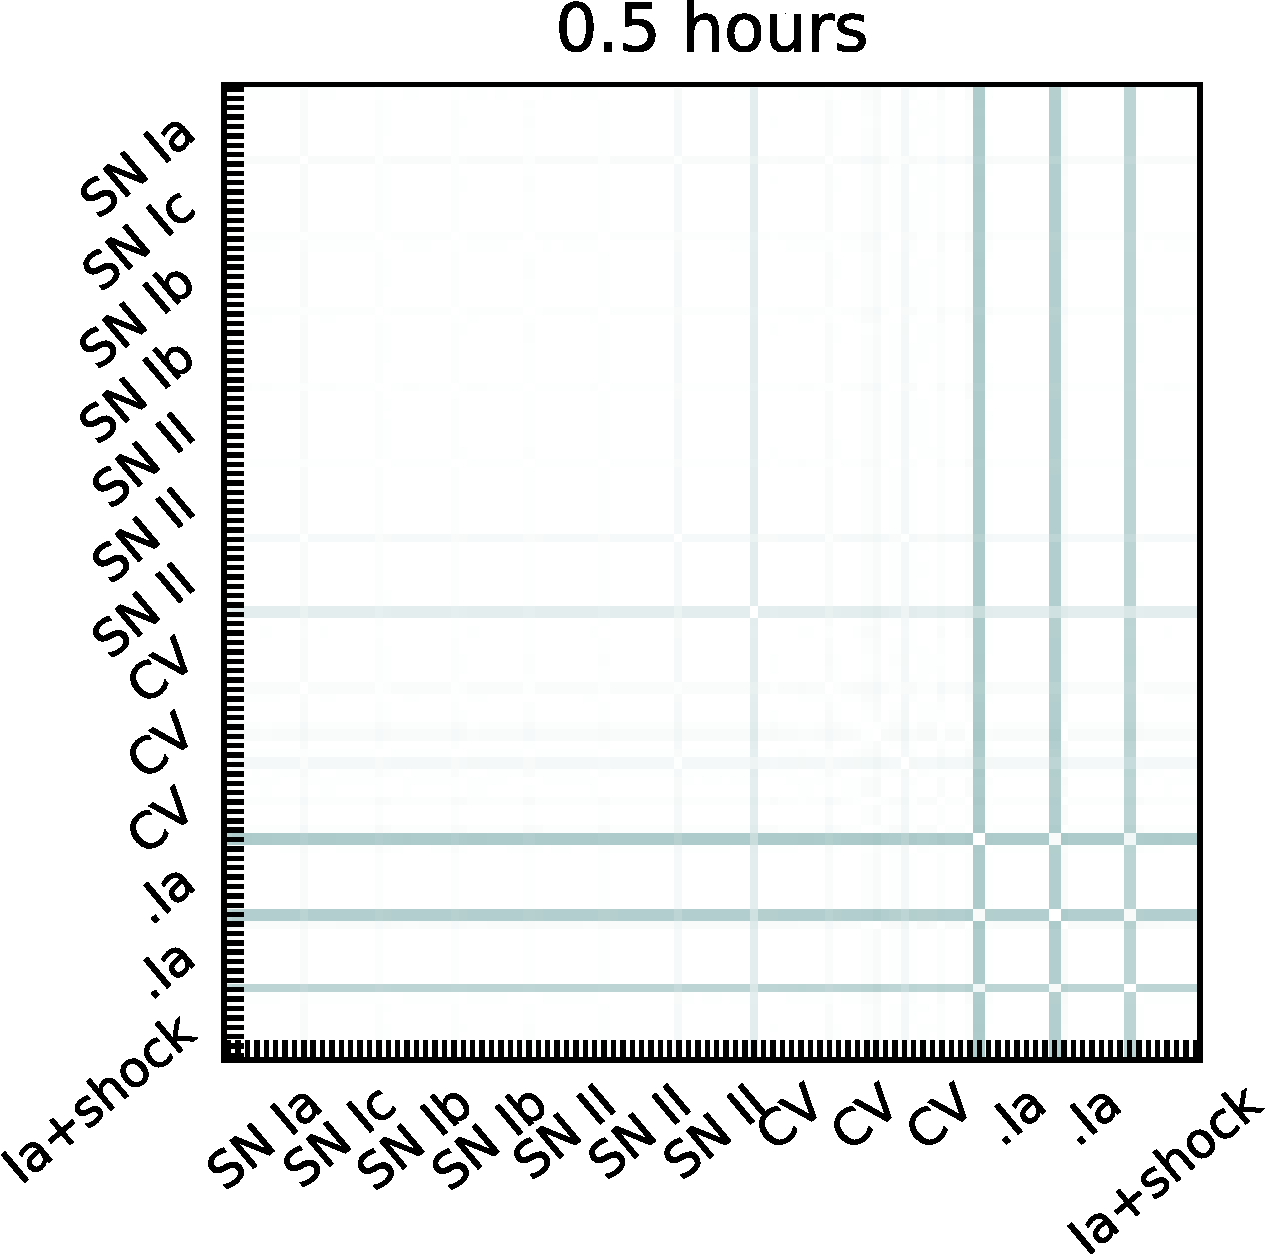
\includegraphics[width=0.8\textwidth]{figs/transients/TransientsAgeSimilarity1.pdf}
    \end{subfigure}%
    ~ 
    \begin{subfigure}[t]{0.45\textwidth}
        \centering
        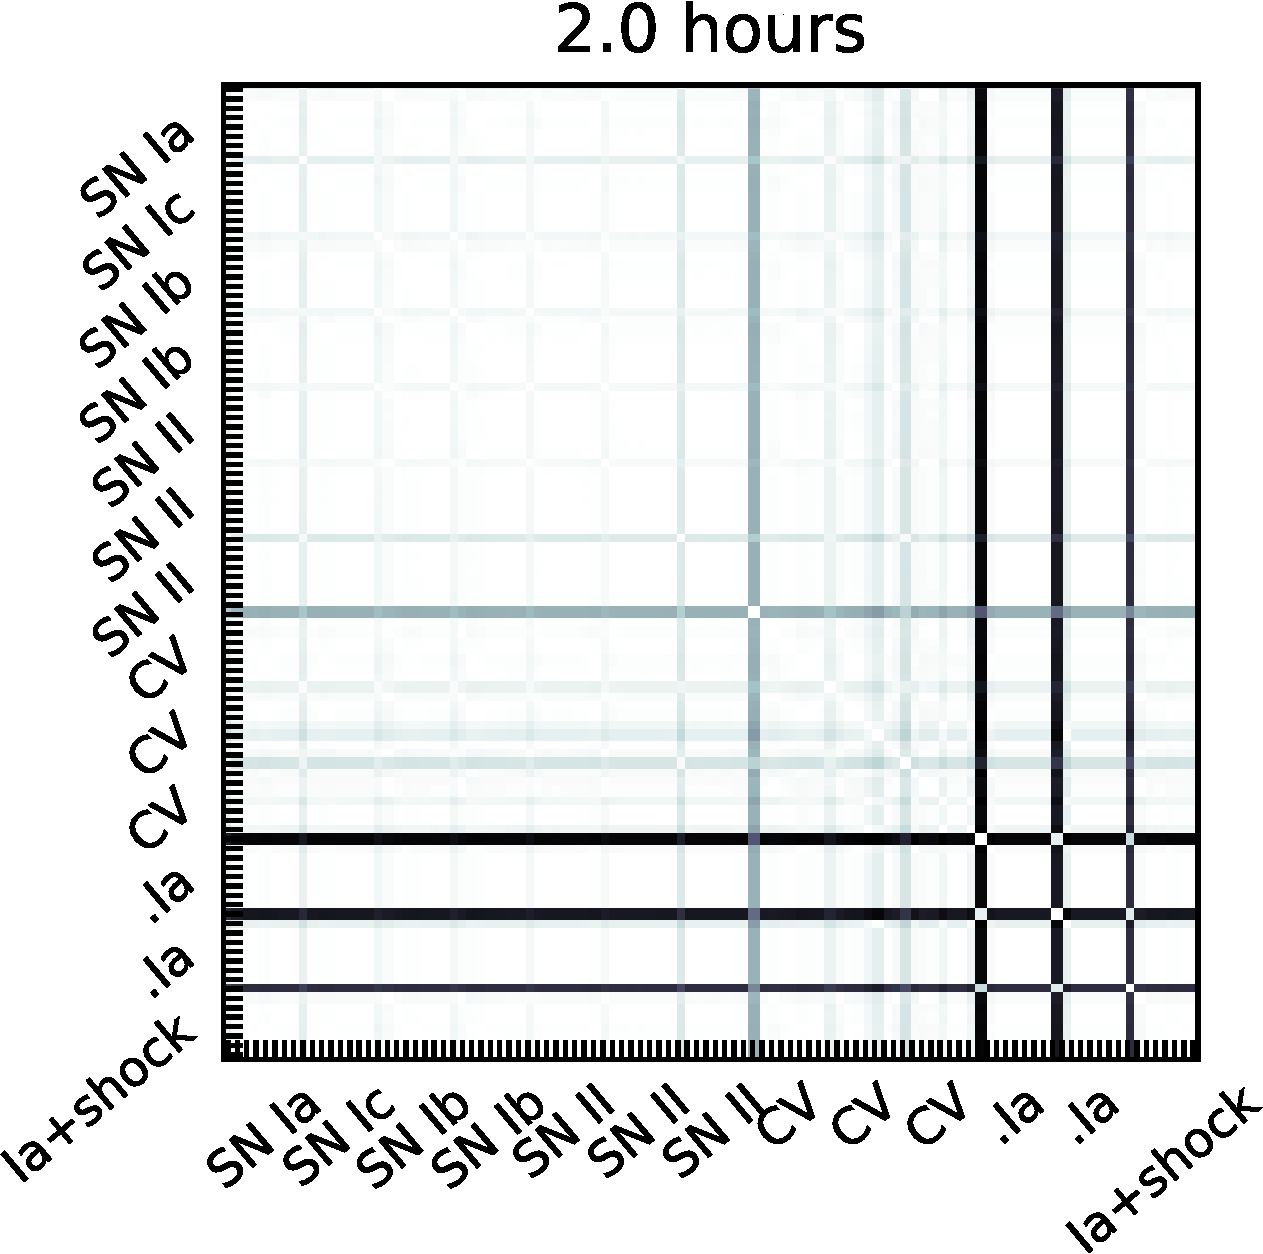
\includegraphics[width=0.8\textwidth]{figs/transients/TransientsAgeSimilarity2.pdf}
    \end{subfigure}


    \begin{subfigure}[t]{0.45\textwidth}
        \centering
        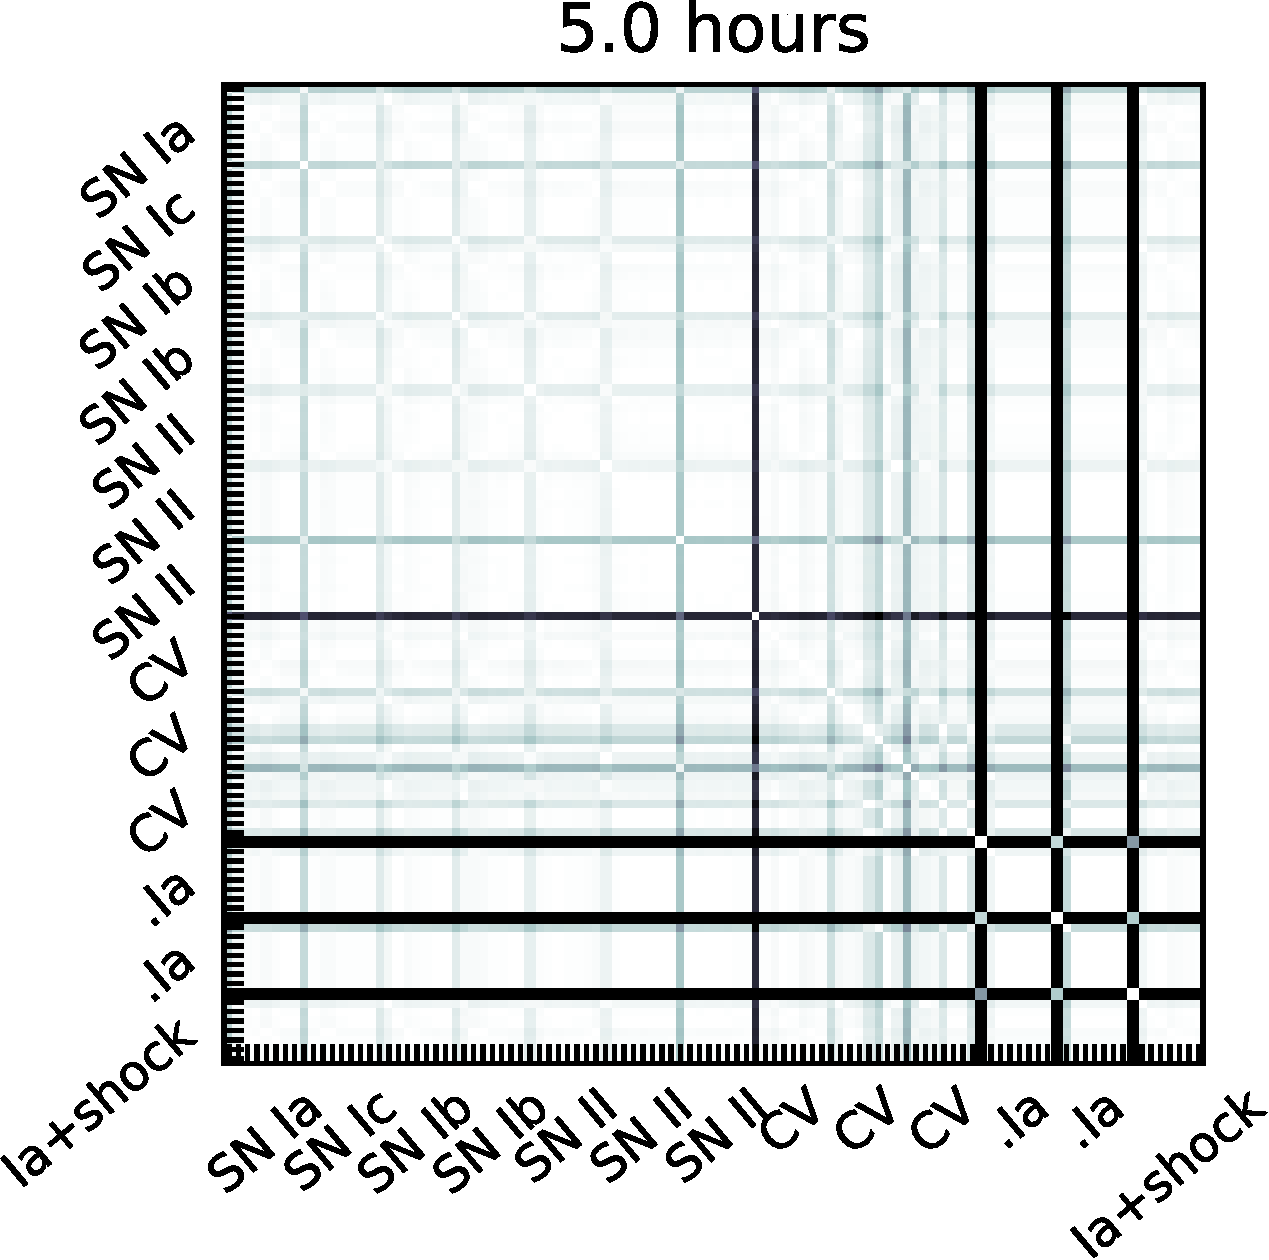
\includegraphics[width=0.8\textwidth]{figs/transients/TransientsAgeSimilarity3.pdf}
    \end{subfigure}%
    ~ 
    \begin{subfigure}[t]{0.45\textwidth}
        \centering
        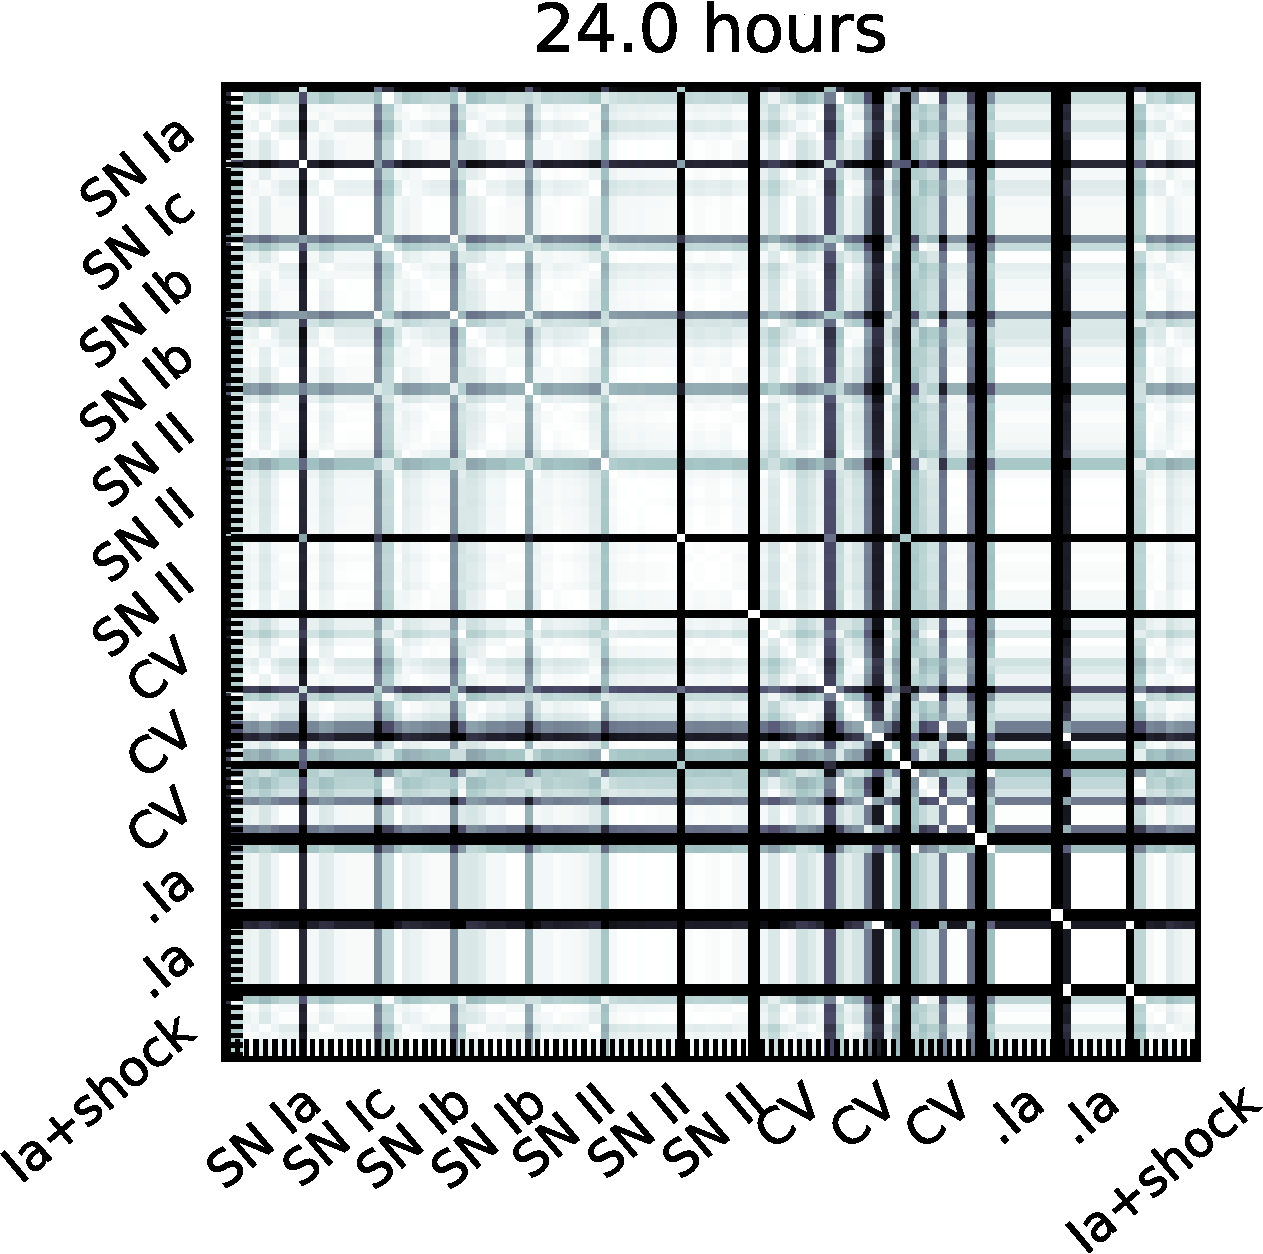
\includegraphics[width=0.8\textwidth]{figs/transients/TransientsAgeSimilarity4.pdf}
    \end{subfigure}
    
%  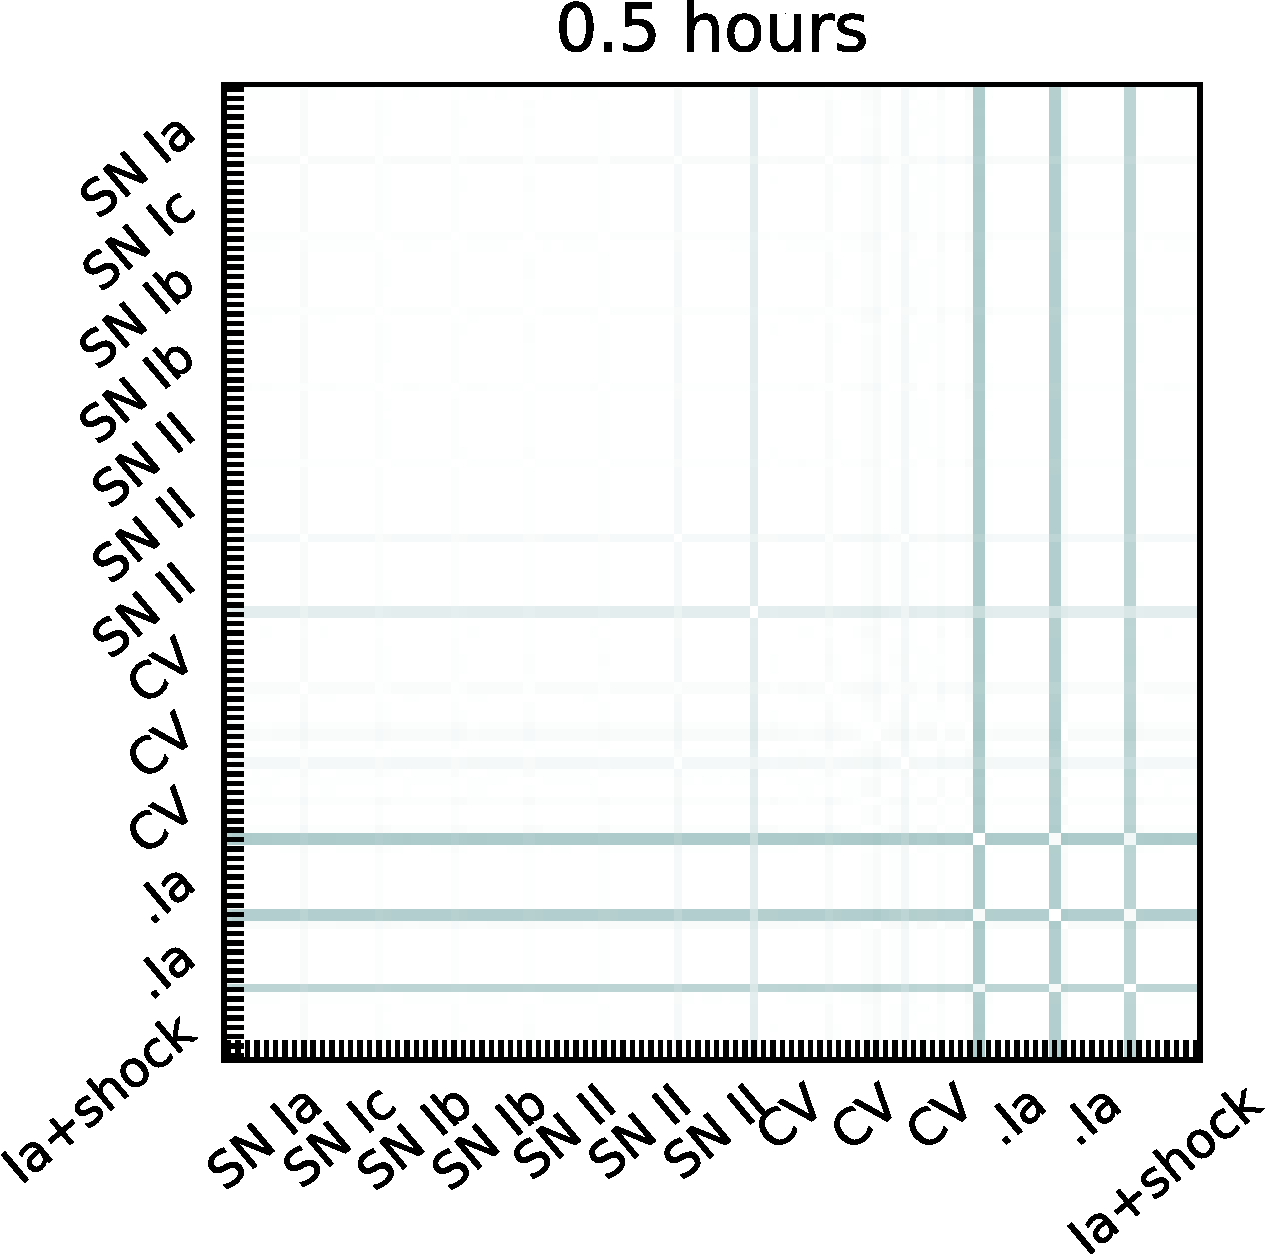
\includegraphics[width=\textwidth]{figs/transients/TransientsAgeSimilarity1.pdf}{figs/transients/TransientsAgeSimilarity2.pdf}
  
    %  \includegraphics[width=\textwidth]{figs/transients/TransientsAgeSimilarit3.pdf}{figs/transients/TransientsAgeSimilarity4.pdf}
    
  
    \caption{Similarity matrix of the transients in \autoref{fig:earlyslope} and \autoref{fig:earlyrise} in $r$ filter for time gaps (starting with the top left panel) of  0.5, 2, 5, and 24 hours.  The similarity is measured as the Euclidean distance between the magnitude change of each transient's pair and it is represented in log scale, with darker colors indicating a larger distance (to a maximum difference $\lvert{\Delta\mathrm{Mag}_1 - \Delta\mathrm{Mag}_2}\rvert ~\sim~8$). For each transient's pair the similarity is calculated for 8 phases within the life of the transients, with the first observation starting at explosion, and as late as 3.5 days after explosion, in 12 hour increments, thus 8 values are associated to each trsansient pair (as indicated by the tick markers).}
  \label{fig:simmatrix}
\end{figure}

% ====================================================================

 \subsection{Conclusions}

 Here we answer the ten questions posed in
 \autoref{sec:intro:evaluation:caseConclusions}:

 \begin{description}

 \item[Q1:] {\it Does the science case place any constraints on the
 tradeoff between the sky coverage and coadded depth? For example, should
 the sky coverage be maximized (to $\sim$30,000 deg$^2$, as e.g., in
 Pan-STARRS) or the number of detected galaxies (the current baseline but
 with 18,000 deg$^2$)?}

 \item[A1:] No strong constraint, as long as larger sky coverage does not compete with dense cadences
required for fast transients.

 \item[Q2:] {\it Does the science case place any constraints on the
 tradeoff between uniformity of sampling and frequency of  sampling? For
 example, a rolling cadence can provide enhanced sample rates over a part
 of the survey or the entire survey for a designated time at the cost of
 reduced sample rate the rest of the time (while maintaining the nominal
 total visit counts).}

 \item[A2:] Frequency of sampling is far more important than uniformity of sampling for early classification of interesting cadence. The rolling cadence is definitely the first step to take, but it is still not enough to identify young transients. A longer than .4 hours intra-night gap or, even better a one day cadence would allow young transients to vary enough to be identified. If the second visit occurs on 0.4-hour time scale, a different filter would be preferred (color information can be alternatively used to identify young transients)
   

 \item[Q3:] {\it Does the science case place any constraints on the
 tradeoff between the single-visit depth and the number of visits
 (especially in the $u$-band where longer exposures would minimize the
 impact of the readout noise)?}

 \item[A3:] Anything that reduces the number of visits per field potentially compromises the objectives.

 \item[Q4:] {\it Does the science case place any constraints on the
 Galactic plane coverage (spatial coverage, temporal sampling, visits per
 band)?}

 \item[A4:] The requirement for multiple visits/filters per night applies to all fields.

 \item[Q5:] {\it Does the science case place any constraints on the
 fraction of observing time allocated to each band?}

 \item[A5:] No.

 \item[Q6:] {\it Does the science case place any constraints on the
 cadence for deep drilling fields?}

 \item[A6:] As discussed in detail above, short bursts of visits separated by several days is not
satisfactory - deep drilling cadences can be devised to provide excellent sampling.

 \item[Q7:] {\it Assuming two visits per night, would the science case
 benefit if they are obtained in the same band or not?}

 \item[A7:] If two visits only, different filters may be the most effective. If more than two visits, the most closely spaced pair should be in the same filter, and the other visits should include at least one other filter.

 \item[Q8:] {\it Will the case science benefit from a special cadence
 prescription during commissioning or early in the survey, such as:
 acquiring a full 10-year count of visits for a small area (either in all
 the bands or in a  selected set); a greatly enhanced cadence for a small
 area?}

 \item[A8:] A greatly enhanced cadence would provide a strong test of the methodology and would jump-start the science.

 \item[Q9:] {\it Does the science case place any constraints on the
 sampling of observing conditions (e.g., seeing, dark sky, airmass),
 possibly as a function of band, etc.?}

 \item[A9:] None unique to transients.

 \item[Q10:] {\it Does the case have science drivers that would require
 real-time exposure time optimization to obtain nearly constant
 single-visit limiting depth?}

 \item[A10:] No.

 \end{description}
